\documentclass{standalone}
\usepackage{graphicx}	
\usepackage{amssymb, amsmath}
\usepackage{color}
\usepackage{wasysym}

\usepackage{tikz}
\usetikzlibrary{intersections, backgrounds}
\usepackage{pgfmath}

\definecolor{light}{RGB}{220, 188, 188}
\definecolor{mid}{RGB}{185, 124, 124}
\definecolor{dark}{RGB}{143, 39, 39}
\definecolor{highlight}{RGB}{180, 31, 180}
\definecolor{gray10}{gray}{0.1}
\definecolor{gray20}{gray}{0.2}
\definecolor{gray30}{gray}{0.3}
\definecolor{gray40}{gray}{0.4}
\definecolor{gray60}{gray}{0.6}
\definecolor{gray70}{gray}{0.7}
\definecolor{gray80}{gray}{0.8}
\definecolor{gray90}{gray}{0.9}
\definecolor{gray95}{gray}{0.95}

\newcommand*{\offset}{0.025}

\begin{document}

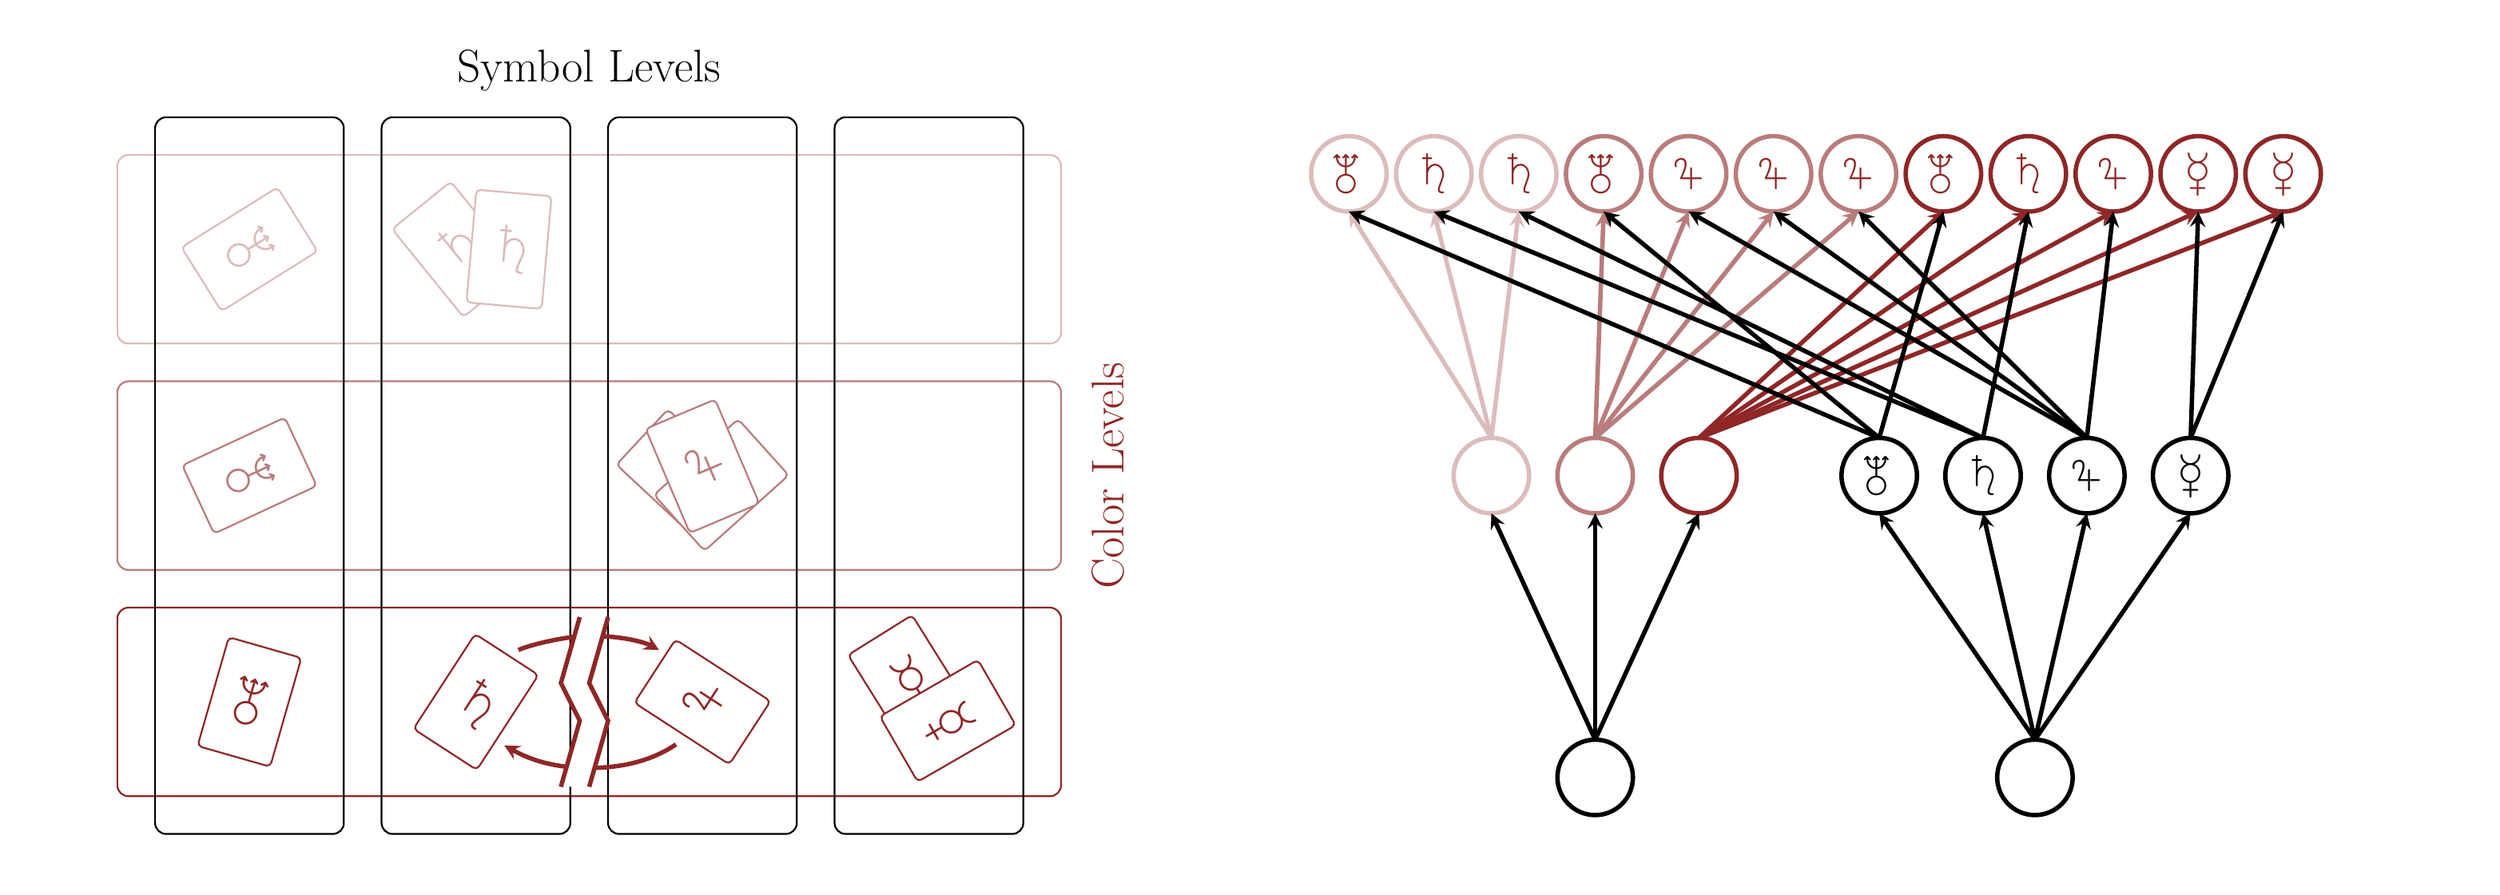
\begin{tikzpicture}[scale=0.3, thick]

\pgfmathsetmacro{\cx}{2}
\pgfmathsetmacro{\cy}{3}

\draw[white] (-30, -21) rectangle (100, 24);

\node[dark, rotate=90] at (27.5, 0) { \huge Color Levels };
\node[black] at (0, 21.5) { \huge Symbol Levels };

\draw[light, rounded corners=5] (-25, 12 - 5) rectangle (25, 12 + 5);
\draw[mid, rounded corners=5] (-25, 0 - 5) rectangle (25, 0 + 5);
\draw[dark, rounded corners=5] (-25, -12 - 5) rectangle (25, -12 + 5);

\draw[black, rounded corners=5] (-18 - 5, -19) rectangle (-18 + 5, 19);
\draw[black, rounded corners=5] (-6 - 5, -19) rectangle (-6 + 5, 19);
\draw[black, rounded corners=5] (6 - 5, -19) rectangle (6 + 5, 19);
\draw[black, rounded corners=5] (18 - 5, -19) rectangle (18 + 5, 19);

% Row One
\pgfmathsetmacro{\phi}{-58}
\pgfmathsetmacro{\x}{-18}
\pgfmathsetmacro{\y}{12}
\begin{scope}[shift={(\x, \y)}, rotate={\phi}]
  \filldraw[fill=white, draw=light, rounded corners=2] (0 - \cx, 0 - \cy) rectangle (0 + \cx, 0 + \cy);
  \node[light, rotate={\phi}] at (0.17, 0) { $\Huge \neptune$ }; 
\end{scope}

\pgfmathsetmacro{\phi}{39}
\pgfmathsetmacro{\x}{-7}
\pgfmathsetmacro{\y}{12}
\begin{scope}[shift={(\x, \y)}, rotate={\phi}]
  \filldraw[fill=white, draw=light, rounded corners=2] (0 - \cx, 0 - \cy) rectangle (0 + \cx, 0 + \cy);
  \node[light, rotate={\phi}] at (0.17, 0) { $\Huge \saturn$ }; 
\end{scope}

\pgfmathsetmacro{\phi}{-5}
\pgfmathsetmacro{\x}{-4.25}
\pgfmathsetmacro{\y}{12}
\begin{scope}[shift={(\x, \y)}, rotate={\phi}]
  \filldraw[fill=white, draw=light, rounded corners=2] (0 - \cx, 0 - \cy) rectangle (0 + \cx, 0 + \cy);
  \node[light, rotate={\phi}] at (0.17, 0) { $\Huge \saturn$ }; 
\end{scope}

% Row Two
\pgfmathsetmacro{\phi}{47}
\pgfmathsetmacro{\x}{6 - 1}
\pgfmathsetmacro{\y}{0}
\begin{scope}[shift={(\x, \y)}, rotate={\phi}]
  \filldraw[fill=white, draw=mid, rounded corners=2] (0 - \cx, 0 - \cy) rectangle (0 + \cx, 0 + \cy);
  \node[mid, rotate={\phi}] at (0.17, 0) { $\Huge \jupiter$ }; 
\end{scope}

\pgfmathsetmacro{\phi}{-65}
\pgfmathsetmacro{\x}{-18}
\pgfmathsetmacro{\y}{0}
\begin{scope}[shift={(\x, \y)}, rotate={\phi}]
  \filldraw[fill=white, draw=mid, rounded corners=2] (0 - \cx, 0 - \cy) rectangle (0 + \cx, 0 + \cy);
  \node[mid, rotate={\phi}] at (0.17, 0) { $\Huge \neptune$ }; 
\end{scope}

\pgfmathsetmacro{\phi}{-48}
\pgfmathsetmacro{\x}{6 + 1}
\pgfmathsetmacro{\y}{0 - 0.5}
\begin{scope}[shift={(\x, \y)}, rotate={\phi}]
  \filldraw[fill=white, draw=mid, rounded corners=2] (0 - \cx, 0 - \cy) rectangle (0 + \cx, 0 + \cy);
  \node[mid, rotate={\phi}] at (0.17, 0) { $\Huge \jupiter$ }; 
\end{scope}

\pgfmathsetmacro{\phi}{23}
\pgfmathsetmacro{\x}{6}
\pgfmathsetmacro{\y}{0 + 0.5}
\begin{scope}[shift={(\x, \y)}, rotate={\phi}]
  \filldraw[fill=white, draw=mid, rounded corners=2] (0 - \cx, 0 - \cy) rectangle (0 + \cx, 0 + \cy);
  \node[mid, rotate={\phi}] at (0.17, 0) { $\Huge \jupiter$ }; 
\end{scope}

% Row Three
\pgfmathsetmacro{\phi}{-33}
\pgfmathsetmacro{\x}{-6}
\pgfmathsetmacro{\y}{-12}
\begin{scope}[shift={(\x, \y)}, rotate={\phi}]
  \filldraw[fill=white, draw=dark, rounded corners=2] (0 - \cx, 0 - \cy) rectangle (0 + \cx, 0 + \cy);
  \node[dark, rotate={\phi}] at (0.17, 0) { $\Huge \saturn$ }; 
\end{scope}

\pgfmathsetmacro{\phi}{-16}
\pgfmathsetmacro{\x}{-18}
\pgfmathsetmacro{\y}{-12}
\begin{scope}[shift={(\x, \y)}, rotate={\phi}]
  \filldraw[fill=white, draw=dark, rounded corners=2] (0 - \cx, 0 - \cy) rectangle (0 + \cx, 0 + \cy);
  \node[dark, rotate={\phi}] at (0.17, 0) { $\Huge \neptune$ }; 
\end{scope}

\pgfmathsetmacro{\phi}{57}
\pgfmathsetmacro{\x}{6}
\pgfmathsetmacro{\y}{-12}
\begin{scope}[shift={(\x, \y)}, rotate={\phi}]
  \filldraw[fill=white, draw=dark, rounded corners=2] (0 - \cx, 0 - \cy) rectangle (0 + \cx, 0 + \cy);
  \node[dark, rotate={\phi}] at (0.17, 0) { $\Huge \jupiter$ }; 
\end{scope}

\pgfmathsetmacro{\phi}{32}
\pgfmathsetmacro{\x}{18 - 1}
\pgfmathsetmacro{\y}{-12 + 1}
\begin{scope}[shift={(\x, \y)}, rotate={\phi}]
  \filldraw[fill=white, draw=dark, rounded corners=2] (0 - \cx, 0 - \cy) rectangle (0 + \cx, 0 + \cy);
  \node[dark, rotate={\phi}] at (0.17, 0) { $\Huge \mercury$ }; 
\end{scope}

\pgfmathsetmacro{\phi}{-60}
\pgfmathsetmacro{\x}{18 + 1}
\pgfmathsetmacro{\y}{-12 - 1}
\begin{scope}[shift={(\x, \y)}, rotate={\phi}]
  \filldraw[fill=white, draw=dark, rounded corners=2] (0 - \cx, 0 - \cy) rectangle (0 + \cx, 0 + \cy);
  \node[dark, rotate={\phi}] at (0.17, 0) { $\Huge \mercury$ }; 
\end{scope}

%\draw[] (0, -12) circle (6 and 3.5);

\draw[dark, line width=2, ->, >=stealth]
   (-3.75, -9.25) 
   .. controls (-3.25, -9) and (-1.25, -12 + 3.5) 
   .. (0, -12 + 3.5)
   .. controls (2.25, -12 + 3.5) and (3.25, -9)
   .. (3.7, -9.25);

\draw[dark, line width=2, <-, >=stealth] 
  (-4.5, -14.3) 
  .. controls (-3.25, -15) and (-2, -12 + -3.5) 
  .. (0, -12 + -3.5)
  .. controls (2, -12 + -3.5) and (3.5, -12 + -3)
  .. (4.6, -14.25);
  
\fill[white] (-0.5, -7.5) -- (-1.5, -11) -- (-0.5, -13) -- (-1.5, -16.5) --
             (0.0, -16.5) -- (1, -13) -- (0.0, -11) -- (1, -7.5);
\draw[dark, line width=2] (-0.5, -7.5) -- (-1.5, -11) -- (-0.5, -13) -- (-1.5, -16.5);
\draw[dark, line width=2] (1, -7.5) -- (0.0, -11) -- (1, -13) -- (0.0, -16.5);


\pgfmathsetmacro{\r}{2}


\filldraw[fill=white, draw=light, line width=2] (65 - 2.25 - 5 * 4.5, 16) circle (\r)
node[color=dark] { $\huge \neptune$ };

\filldraw[fill=white, draw=light, line width=2] (65 - 2.25 - 4 * 4.5, 16) circle (\r)
node[color=dark] { $\huge \saturn$ };

\filldraw[fill=white, draw=light, line width=2] (65 - 2.25 - 3 * 4.5, 16) circle (\r)
node[color=dark] { $\huge \saturn$ };

\filldraw[fill=white, draw=mid, line width=2] (65 - 2.25 - 2 * 4.5, 16) circle (\r)
node[color=dark] { $\huge \neptune$ };

\filldraw[fill=white, draw=mid, line width=2] (65 - 2.25 - 1 * 4.5, 16) circle (\r)
node[color=dark] { $\huge \jupiter$ };

\filldraw[fill=white, draw=mid, line width=2] (65 - 2.25, 16) circle (\r)
node[color=dark] { $\huge \jupiter$ };

\filldraw[fill=white, draw=mid, line width=2] (65 + 2.25, 16) circle (\r)
node[color=dark] { $\huge \jupiter$ };

\filldraw[fill=white, draw=dark, line width=2] (65 + 2.25 + 1 * 4.5, 16) circle (\r)
node[color=dark] { $\huge \neptune$ };

\filldraw[fill=white, draw=dark, line width=2] (65 + 2.25 + 2 * 4.5, 16) circle (\r)
node[color=dark] { $\huge \saturn$ };

\filldraw[fill=white, draw=dark, line width=2] (65 + 2.25 + 3 * 4.5, 16) circle (\r)
node[color=dark] { $\huge \jupiter$ };

\filldraw[fill=white, draw=dark, line width=2] (65 + 2.25 + 4 * 4.5, 16) circle (\r)
node[color=dark] { $\huge \mercury$ };

\filldraw[fill=white, draw=dark, line width=2] (65 + 2.25 + 5 * 4.5, 16) circle (\r)
node[color=dark] { $\huge \mercury$ };


\draw[->, >=stealth, color=light, line width=2] (53.3 - 5.5, 0 + \r) -- (65 - 2.25 - 5 * 4.5, 16 - \r);
\draw[->, >=stealth, color=light, line width=2] (53.3 - 5.5, 0 + \r) -- (65 - 2.25 - 4 * 4.5, 16 - \r);
\draw[->, >=stealth, color=light, line width=2] (53.3 - 5.5, 0 + \r) -- (65 - 2.25 - 3 * 4.5, 16 - \r);

\filldraw[fill=white, draw=light, line width=2] (53.3 - 5.5, 0) circle (\r);

\draw[->, >=stealth, color=mid, line width=2] (53.3, 0 + \r) -- (65 - 2.25 - 2 * 4.5, 16 - \r);
\draw[->, >=stealth, color=mid, line width=2] (53.3, 0 + \r) -- (65 - 2.25 - 1 * 4.5, 16 - \r);
\draw[->, >=stealth, color=mid, line width=2] (53.3, 0 + \r) -- (65 - 2.25, 16 - \r);
\draw[->, >=stealth, color=mid, line width=2] (53.3, 0 + \r) -- (65 + 2.25, 16 - \r);

\filldraw[fill=white, draw=mid, line width=2] (53.3, 0) circle (\r);

\draw[->, >=stealth, color=dark, line width=2] (53.3 + 5.5, 0 + \r) -- (65 + 2.25 + 1 * 4.5, 16 - \r);
\draw[->, >=stealth, color=dark, line width=2] (53.3 + 5.5, 0 + \r) -- (65 + 2.25 + 2 * 4.5, 16 - \r);
\draw[->, >=stealth, color=dark, line width=2] (53.3 + 5.5, 0 + \r) -- (65 + 2.25 + 3 * 4.5, 16 - \r);
\draw[->, >=stealth, color=dark, line width=2] (53.3 + 5.5, 0 + \r) -- (65 + 2.25 + 4 * 4.5, 16 - \r);
\draw[->, >=stealth, color=dark, line width=2] (53.3 + 5.5, 0 + \r) -- (65 + 2.25 + 5 * 4.5, 16 - \r);

\filldraw[fill=white, draw=dark, line width=2] (53.3 + 5.5, 0) circle (\r);

\draw[->, >=stealth, color=black, line width=2] (53.3, -16 + \r) -- (53.3 - 5.5, 0 - \r);
\draw[->, >=stealth, color=black, line width=2] (53.3, -16 + \r) -- (53.3, 0 - \r);
\draw[->, >=stealth, color=black, line width=2] (53.3, -16 + \r) -- (53.3 + 5.5, 0 - \r);

\filldraw[fill=white, draw=black, line width=2] (53.3, -16) circle (\r);


\draw[->, >=stealth, color=black, line width=2] (76.6 - 8.25, 0 + \r) -- (65 - 2.25 - 5 * 4.5, 16 - \r);
\draw[->, >=stealth, color=black, line width=2] (76.6 - 8.25, 0 + \r) -- (65 - 2.25 - 2 * 4.5, 16 - \r);
\draw[->, >=stealth, color=black, line width=2] (76.6 - 8.25, 0 + \r) -- (65 - 2.25 + 2 * 4.5, 16 - \r);

\filldraw[fill=white, draw=black, line width=2] (76.6 - 8.25, 0) circle (\r)
node[color=black] { $\huge \neptune$ };

\draw[->, >=stealth, color=black, line width=2] (76.6 - 2.75, 0 + \r) -- (65 - 2.25 - 4 * 4.5, 16 - \r);
\draw[->, >=stealth, color=black, line width=2] (76.6 - 2.75, 0 + \r) -- (65 - 2.25 - 3 * 4.5, 16 - \r);
\draw[->, >=stealth, color=black, line width=2] (76.6 - 2.75, 0 + \r) -- (65 + 2.25 + 2 * 4.5, 16 - \r);

\filldraw[fill=white, draw=black, line width=2] (76.6 - 2.75, 0) circle (\r)
node[color=black] { $\huge \saturn$ };

\draw[->, >=stealth, color=black, line width=2] (76.6 + 2.75, 0 + \r) -- (65 - 2.25 - 1 * 4.5, 16 - \r);
\draw[->, >=stealth, color=black, line width=2] (76.6 + 2.75, 0 + \r) -- (65 - 2.25, 16 - \r);
\draw[->, >=stealth, color=black, line width=2] (76.6 + 2.75, 0 + \r) -- (65 + 2.25, 16 - \r);
\draw[->, >=stealth, color=black, line width=2] (76.6 + 2.75, 0 + \r) -- (65 + 2.25 + 3 * 4.5, 16 - \r);

\filldraw[fill=white, draw=black, line width=2] (76.6 + 2.75, 0) circle (\r)
node[color=black] { $\huge \jupiter$ };

\draw[->, >=stealth, color=black, line width=2] (76.6 + 8.25, 0 + \r) -- (65 + 2.25 + 4 * 4.5, 16 - \r);
\draw[->, >=stealth, color=black, line width=2] (76.6 + 8.25, 0 + \r) -- (65 + 2.25 + 5 * 4.5, 16 - \r);

\filldraw[fill=white, draw=black, line width=2] (76.6 + 8.25, 0) circle (\r)
node[color=black] { $\huge \mercury$ };

\draw[->, >=stealth, color=black, line width=2] (76.6, -16 + \r) -- (76.6 - 8.25, 0 - \r);
\draw[->, >=stealth, color=black, line width=2] (76.6, -16 + \r) -- (76.6 - 2.75, 0 - \r);
\draw[->, >=stealth, color=black, line width=2] (76.6, -16 + \r) -- (76.6 + 2.75, 0 - \r);
\draw[->, >=stealth, color=black, line width=2] (76.6, -16 + \r) -- (76.6 + 8.25, 0 - \r);

\filldraw[fill=white, draw=black, line width=2] (76.6, -16) circle (\r);


\end{tikzpicture}

\end{document}  